\documentclass{article}
\usepackage{tikz}
\usetikzlibrary{automata, positioning, arrows.meta, shapes}

\begin{document}

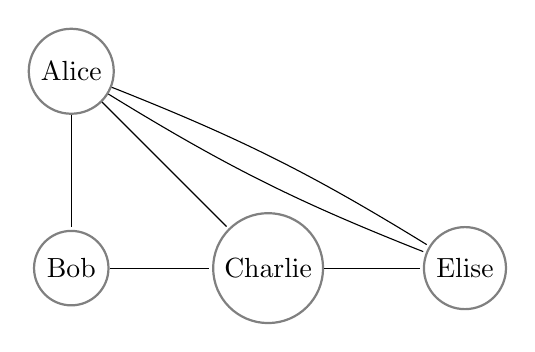
\begin{tikzpicture}[shorten >=1pt, node distance=2.5cm, on grid, auto,
    every state/.style={draw=black!50, thick, minimum size=0.8cm, inner sep=3pt},
    edge_label/.style={midway, fill=white, inner sep=1pt, font=\small}
]

% Graph Definition
    \node[state] (Alice) {Alice};
    \node[state] (Bob) [below=of Alice] {Bob};
    \node[state] (Charlie) [right=of Bob] {Charlie};
    \node[state] (Elise) [right=of Charlie] {Elise};

% Edges
    \path[-] (Alice) edge[bend left=0] (Bob);
    \path[-] (Alice) edge[bend left=0] (Charlie);
    \path[-] (Alice) edge[bend right=5] (Elise);
    \path[-] (Alice) edge[bend left=5] (Elise);
    \path[-] (Bob) edge[bend left=0] (Charlie);
    \path[-] (Charlie) edge[bend left=0] (Elise);

\end{tikzpicture}

\end{document}
